\section{System Overview}

Motivated by outliers problem, we named our system for NO Outliers ($NO^2$) expressed our best wishes and indicated $NO^2$'s mission. As far as we know, the only one system have a similar name with $NO^2$ in the world, called N2O system, is primarily concerned with introducing fuel and nitrous into the engine's cylinders, and combining them for more efficient combustion. It is typically used to provide an instantaneously speedup for auto, while our $NO^2$ system can persistently speeding up parallel processing for massive compute-intensive tasks in clusters and clouds.

$NO^2$ contains two main components, the instrumenter and tasks scheduling policy generater. The instrumenter has a perfect partner, the instrument points selector, which collects the statistics of function hits in a variety of executions and select some function entries for a appropriate instrumentation granularity. Though the instrumenter can finish the instrument task for tracing progress itself, an additional overhead as much as several percentages of execution time is unavoidable. This is unacceptable in production system, but with the instrument points selector's cooperation, overheads can be cut down to little, even negligible. Details will be shown in the evaluation section. The tasks scheduling policy generater is supported by the outliers clustering. With the outliers information, an optimized tasks scheduling policy can be generated for the job running on cluster.

\begin{figure}
\centering
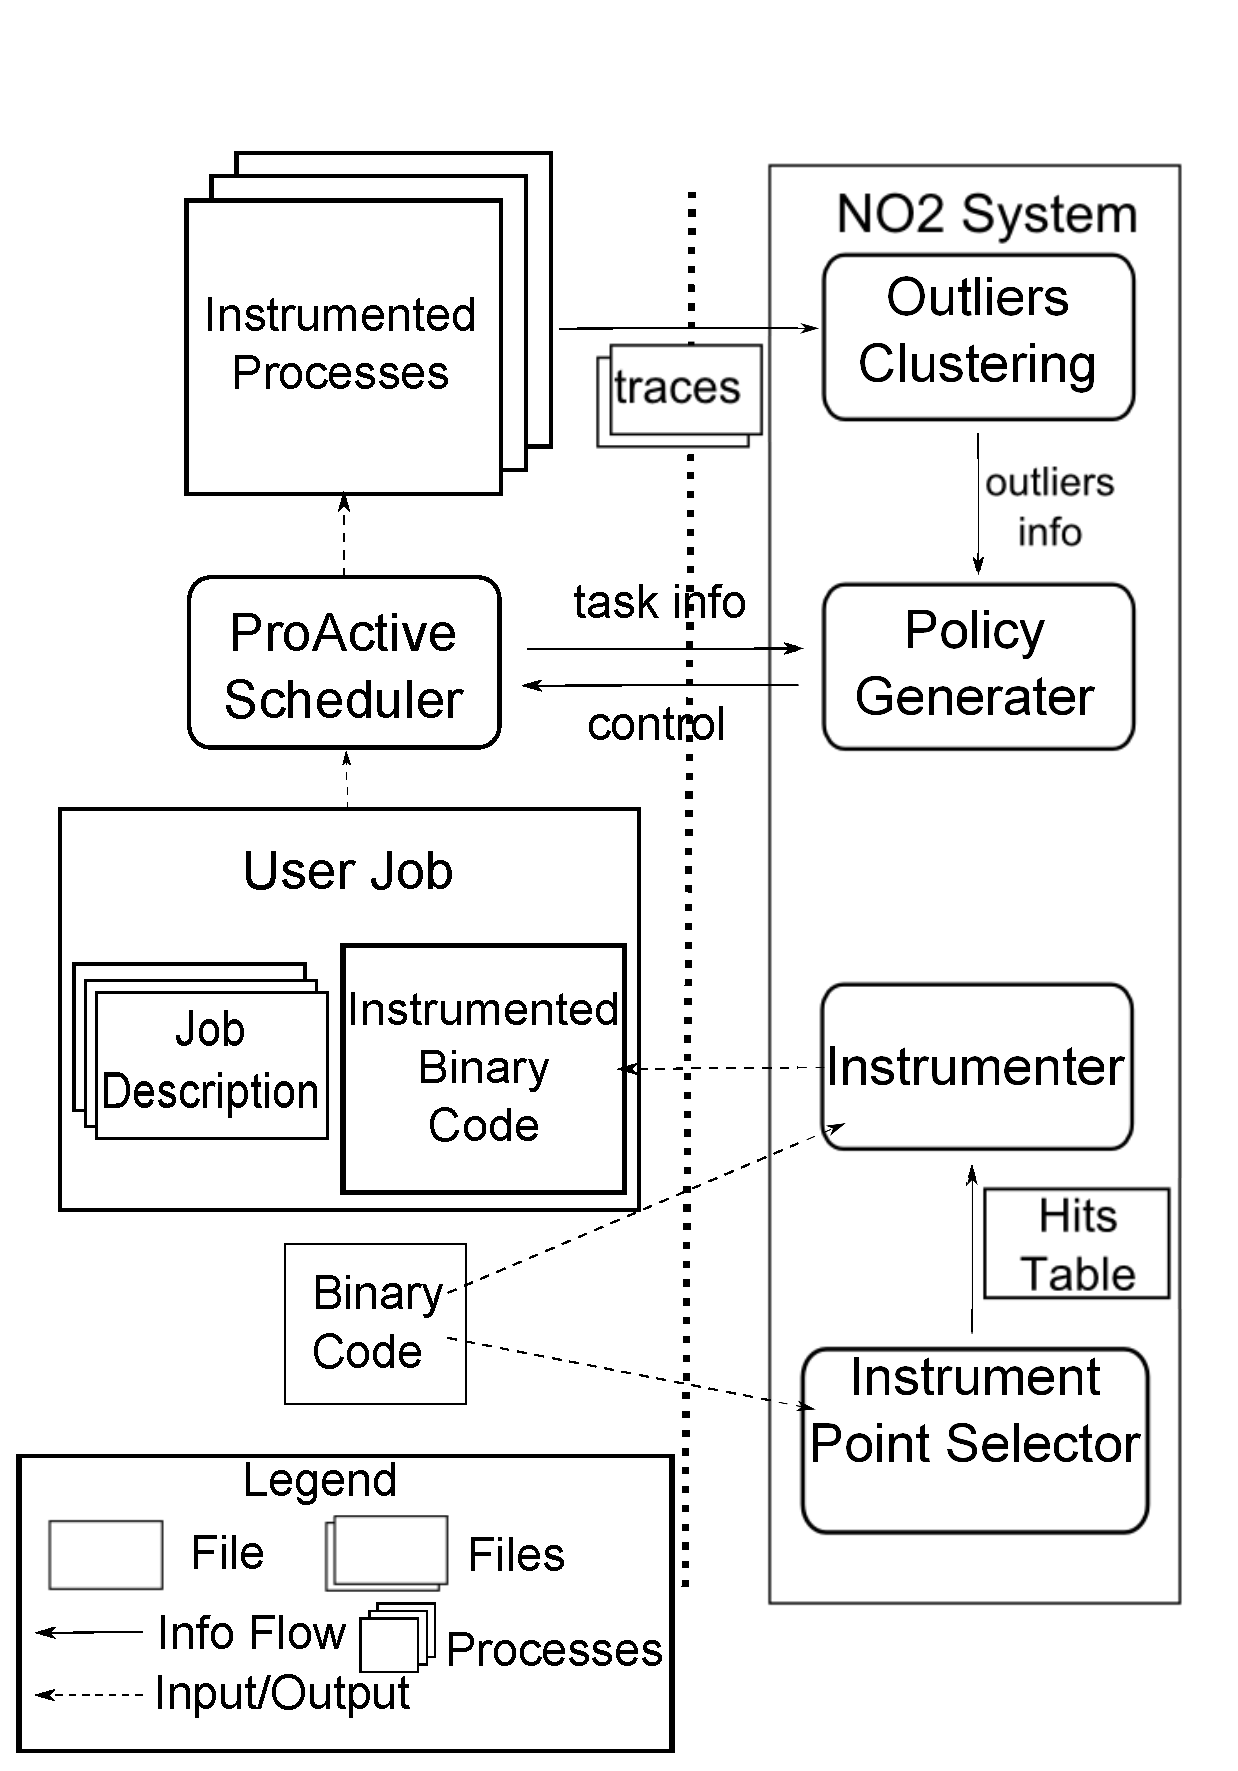
\includegraphics[width=0.9\columnwidth]{figures/NO2_arch.eps}
\caption{$NO^2$ Architecture}
\label{figure:no2arch}
\end{figure}

We carefully designed $NO^2$ to make sure of its independence with job scheduler which benefits users adapting to different job schedulers easily. As Fig. \ref{figure:no2arch} shows, the only interactive is the interface between $NO^2$ and ProActive Scheduler. The interface is for obtaining task status information of a job and requesting to kill or start a task. These abilities can be easily satisfied by any job scheduler's control interface, such as control script provided by ProActive Scheduler or command line tools provided by Condor.

The instrumentation has two phases: function hits statistics and instrument with selected functions by the instrument points selector. For function hit statistics, another instrumentation is needed. As the statistics is offline, this instrumentation covers all functions in the binary code with no need to considering instrumentation overhead. The modified binary code runs with some input cases usually executed in realistic and saves the statistics results in a file. With the statistics, An instrumentation for progress trace can be performed with the binary code in a appropriate granularity.

The speculation algorithm of tasks scheduling for a job is straightforward with a few of heuristics improvement driven by several rules of thumb. These empirical rules are reasonable and verified in practice. The first rule is giving worst guy of outliers more speculation priority. As speculation is not completely free, it is obviously advisable. Making sure of the split task and merge task not executing on irregular nodes is another important rule because of the impossible of exposing outlier with single task. On the other hand, the split and merge phases are always in the critical path of a job. The last one is speculation as soon as possible without irregular nodes. As the goal of speculation is early completion of job, speculation earlier and faster means better opportunity. The pseudo code of speculation algorithm is show in Fig. \ref{fig-spec-algo}.

\begin{figure}
\rule[-.2pt]{0.9\columnwidth}{0.9pt}
\textbf{Algorithm:TasksSpeculation}
\rule[-.2pt]{0.9\columnwidth}{0.5pt}

\begin{algorithmic}[1]
\Require{instance of the $job$ and sleep $interval$}
\Ensure{the job's state $job.state$}




\While{$job.state\not=FinishedOrFaulty$}
    \State $tasks\gets job.tasks$
    \State $clusters\gets kmeans(tasks.traces, 2)$
    \If{$variance(clusters) > threshold$}
        \State $outliers\gets min(clusters)$
        \State $sort(outliers, comparePriority)$
        \For{$outlier \in outliers$}
            \State $s\gets submit(outlier.taskid)$
            \State $speculations\gets [speculations, s]$
        \EndFor
    \EndIf
    \State $sleep(interval)$
    \State $job.update()$
    \For{$s \in speculations$}
        \If{$s.state = Finished$}
            \State $kill(s.outlier.taskid)$
        \ElsIf{$s.outlier.state = Finished$}
            \State $kill(s.taskid)$
        \EndIf
    \EndFor
\EndWhile\label{specendwhile}
\end{algorithmic}
\rule[-.2pt]{0.9\columnwidth}{0.8pt}
\caption{Tasks Speculation Algorithm}\label{fig-spec-algo}
\end{figure}

In the next two sections, we will mainly illustrate the design of instrumentation based on function hits statistics and outliers clustering, two key points in $NO^2$ system. 